\documentclass[tikz,border=3pt]{standalone}
\usepackage{amsmath}
\usepackage{tikz}
\usetikzlibrary{shapes.geometric,arrows.meta,patterns,calc,decorations.pathreplacing}

\begin{document}
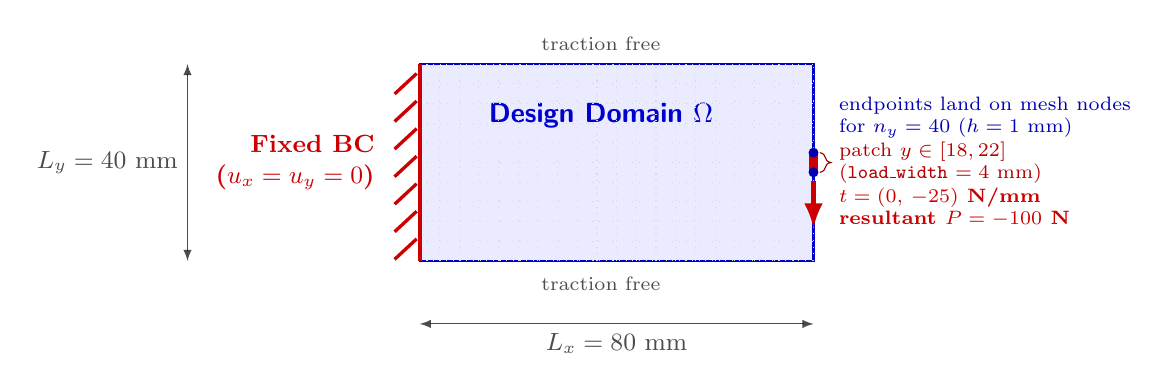
\begin{tikzpicture}[scale=1.0, >=latex]
  % CantileverMiddle2d: 80 x 40 mm, 绘图比例 0.0625 -> 5.0 x 2.5
  % 载荷区 y in [18, 22] (load_width = 4 mm) -> 绘图 y in [1.125, 1.375]
  % Design Domain
  \draw[thick, fill=blue!8, draw=blue!80!black] (0,0) rectangle (5,2.5);
  \node[font=\bfseries\sffamily, color=blue!80!black] at (2.3,1.85) {Design Domain $\Omega$};

  % Grid overlay
  \draw[step=0.25, gray!30, dotted] (0,0) grid (5,2.5);

  % Fully clamped Left Boundary (x = 0): u_x = u_y = 0
  \draw[ultra thick, red!80!black] (0,0) -- (0,2.5);
  \foreach \y in {0.15, 0.5, 0.85, 1.2, 1.55, 1.9, 2.25} {
    \draw[line width=1.2pt, red!80!black] (-0.32, \y-0.13) -- (-0.04, \y+0.13);
  }
  \node[left, red!80!black, font=\small\bfseries, align=right] at (-0.45,1.25)
    {Fixed BC\\($u_x = u_y = 0$)};

  % Load patch on the Right Boundary (x = 80), y in [18, 22]
  \draw[line width=3.5pt, red!80!black] (5,1.125) -- (5,1.375);
  \fill[blue!70!black] (5,1.125) circle (1.8pt);
  \fill[blue!70!black] (5,1.375) circle (1.8pt);
  \draw[decorate, decoration={brace, amplitude=4pt}, red!60!black]
    (5.08,1.375) -- (5.08,1.125);

  % Traction direction: tangential (downward) on the end face
  \draw[->, ultra thick, red!80!black, line width=2pt] (5.0,1.02) -- (5.0,0.42);

  % 右侧标注自上而下: 端点对齐 / 载荷区范围 / 牵引强度
  \node[right, blue!70!black, font=\scriptsize, align=left] at (5.2,1.82)
    {endpoints land on mesh nodes\\for $n_y = 40$ ($h = 1$ mm)};
  \node[right, red!70!black, font=\scriptsize, align=left] at (5.2,1.25)
    {patch $y \in [18, 22]$\\(\texttt{load\_width} $= 4$ mm)};
  \node[right, red!80!black, font=\scriptsize\bfseries, align=left] at (5.2,0.68)
    {$t = (0,\,-25)\text{ N/mm}$\\resultant $P = -100\text{ N}$};

  % Traction-free top and bottom
  \node[above, gray!60!black, font=\scriptsize] at (2.3,2.55) {traction free};
  \node[below, gray!60!black, font=\scriptsize] at (2.3,-0.08) {traction free};

  % Dimensions
  \draw[<->, opacity=0.7] (0,-0.8) -- (5,-0.8) node[midway, below, font=\small] {$L_x = 80\text{ mm}$};
  \draw[<->, opacity=0.7] (-2.95,0) -- (-2.95,2.5) node[midway, left, font=\small] {$L_y = 40\text{ mm}$};
\end{tikzpicture}
\end{document}
